\chapter{Introduction}

The growing needs for information availability and accessibility present new challenges for application development. Stand-alone applications cannot fulfil the growing needs anymore. There are two forces working in parallel with regard to the need for integration. First, it is necessary to allow for application integration within an enterprise, and second, there are growing needs to ensure inter-enterprise or ``business-to-business'' integration.

The majority of companies, however, still have existing legacy applications, developed using different architectures and technologies, which have usually not been designed for integration. Companies cannot afford to write off or replace them over night, because they are mission critical; also they cannot afford to develop their entire information systems from scratch in today's business environment.

In addition, companies will undoubtedly need to introduce new applications and systems from time to time. New solutions are usually based on modern architectures, which differ significantly from architectures used by existing legacy applications. These new applications also have to be integrated with existing applications; and existing applications have to be integrated with each other to fulfil the information availability and accessibility goals. To make things even more difficult, there is often a significant investment already in place for a variety of application integration technologies.

It can be clearly seen that integrating applications is a difficult task, may be even one of the most difficult problems facing enterprise application development. To fulfil these integration objectives, several methods, techniques, patterns, and technologies have been developed over the years, ranging from point-to-point integration over enterprise application integration (EAI) and business process management to service oriented architectures (SOA).

The ability to instantly access vital information that may be stored in a variety of different applications may influence the success of a company. For each company, the presence of effective information infrastructure that avoids the need for employees to perform numerous manual tasks like filling in paper forms, and other bureaucracy, is very important. Employees should not have to contend with such inefficiencies and irritations, such as switching between different applications to get their work done, reentering the same data more than once in different applications, or waiting for data to be processed. Ideally, a well-integrated system should offer \textbf{end-to-end support} for business processes with \textbf{instant} access to information, no matter which part of the system is used. Similar consideration hold true for companies that want to be successful in e-business or those that want to improve their position in the virtual world. 

Companies are realizing the importance of integration at different speeds. Those, who have seen the advantages of integration and understand how to achieve successful integration, are already fully involved in integration projects with many solutions already working. Other companies are aware that integration is important but, although they may have started integration projects, they do not have the results yet, mainly because the integration projects have not been successful. Further still, some companies are only now realizing the importance of integration, and this could in fact be too late for them. Such companies may be looking for ways to achieve integration fast, without spending too much money, and without assigning too many staff members to the integration project. But cutting corners and attempting to implement only the most needed parts of integration in the shortest possible time will most likely result in only partially working solutions at best.

The problem that makes things worse is the fact that \textit{managers are} often \textit{not familiar} with all the complexity hidden behind the integration process. Sometimes, even the ``IT people'', the architects and developers, do not fully understand the traps behind integration. Most importantly, managers might not understand that integration is a topic that is related to the company as a whole, and not with the IT department only.

Another scenario that leads to the same disorganized approach is when the management of a company does not see the need for integration yet, but the IT department is aware that integration is needed and should be initiated as soon as possible. Therefore, the integration team starts to build a partial solution to solve the most urgent problems. As the integration is not approved from the top, the IT sector does not get enough resources, it does not have enough time and money, and, most significantly, it does not have authorization to start to solve the integration problem globally. Most developers will agree that these are all-too-familiar situations.

\textbf{Integration} seems to be one of most important strategic priorities, mainly because new innovative business solutions demand integration of different business units, enterprise data, applications, and business systems. Integrated information systems improve the competitive advantage with unified and efficient access to the information. Integrated applications make it much easier to access relevant, coordinated information from a variety of sources. In effect, the total becomes more than the sum of its parts. It's easy to see that integration can be an important and attractive strategic priority.

Typical companies that have existed more than just a few years rarely have integrated information systems. Rather they are faced with a disparate mix of heterogeneous existing systems. Companies will typically have different applications, developed over time. These include:

\begin{compactenum}
\item  Applications developed inside the company

\item  Custom-built but outsourced solutions

\item  Commercial and ERP applications
\end{compactenum}

These applications have typically been developed on different platforms, using different technologies and programming languages. Because they have been developed over time, different applications use different programming models. This is manifested through:

\begin{compactenum}
\item  Combinations of monolithic, client/server, and multi-tier applications

\item  Mix of procedural, object-oriented, and component-based solutions

\item  Mix of programming languages

\item  Different types of database management systems (relational, hierarchical, object) and products

\item  Different middleware solutions for communication (message-oriented middleware, object request brokers (ORB), remote procedure calls (RPC), etc.)

\item  Multiple information transmission models, including publish/subscribe, request/reply, and conversational

\item  Different transaction and security management middleware

\item  Different ways of sharing data

\item  Possible usage of EDI, XML, and other proprietary formats for data exchange
\end{compactenum}

\section{Problem Definition and Main Challenges}

Another important aspect is the integration that has already been implemented between the existing applications. This includes everything from simple data exchange to use of middleware products. In addition to all this diversity of architectures, technologies, platforms, and programming languages the companies have kept introducing new applications --- and with new applications they have introduced modern application architectures too. 

As it has been said in introduction, Web Services are rapidly increasing in complexity and range due to their wide applicability to internet users and businesses, and the use of XML (Extensive Markup Language) formalizing the description of data exchange. Recently, an effort has been made to control communication between web services with the introduction of new methods such as standardized Business Transaction Protocols. Session-Based programming uses a typing language to achieve that control and is said to be highly suitable for programming web service communication. 

This thesis presents the novel ideas in the form of formal theory of distributed session programming and presents the practical implementation of session-based programming language, shows the main features and compares with already existing solutions. Business transactions in traditional software engineering are understood to be entities with a short life spam operating in a closely coupled context. They are designed for successful completions, without complications such as loss of data arising during exchange. Hence, with minimal control, thousands of transparent transactions can occur within a system every second without troubling the programmer. 

The \textbf{smooth operation of interaction} between web services is, however, much harder to achieve. The reason behind that is that when we try to extend the concept of traditional transactions to a loosely coupled environment such as the web we find that they're unsuitable. The situation becomes even harder if companies are dealing with applications of a long life spam, running for hours or even days and almost inevitably resulting in a deadlock. Business-to-business interactions often require such long-lived transactions. A need arises for new transaction implementations, more suitable for the web.

Protocols already exist but the recent blossoming of web services, combining more and more distributed services makes this a very important topic in today's industrial world. In this project we will be focusing on Session-Based Programming, a method of controlling process interactions (represented by sessions). It works by specifying the intended process transaction protocol using \textit{session types} and implementing the interaction using \textit{session operations}. The session implementations will then be verified with the session specifications to guarantee a correct implementation and secure communication between web services. \textbf{Session-Java} (SJ) is an extension to Java implementing Session-Based Programming. The language, that has been developed by scientific members from Imperial College (London) and Queen Mary University (London), is still under development but a stable version of it exists and by programming in it I have built several real life scenarios of web businesses interacting. Those scenarios can be used by the SJ designers as programming paradigms or compared with similar implementations in other languages such as for example the Java RMI and CORBA. The thesis is focusing basically on business scenarios, although there is a wide enough subspace to test different aspects of the language: parallel algorithms, real-time communication). This will be the first time that business communication of a sufficient depth will be implemented in SJ, so our scenarios aim to test multiple aspects of the language and enable us to identify its pros and cons. Our priority is that by the end of the project we will have produced complicated programs in SJ. Through these we're aiming to confirm the suitability of Session-Java as an implementation of business to business transactions. We want to explore the robustness of the language and the scalability as scenarios vary in size but also complexity. In addition we will be looking for things such as ease of programming in SJ, any limitations, bugs or non-implementable scenarios.

In fact, SJ is closely tied to the Web Services Choreography Working group \cite{comseqpro}, currently designing the Web Services Choreography Description Language (WS-CDL) aimed specifically at interactions amongst web services. The plan is that SJ will be used as part of the implementation technologies for the language. Like UML with Java, this could possibly be directly translated to SJ code, and hence generate code skeletons. If, however, there exist any non-implementable scenarios in SJ then they will have to be overcome before that stage is reached.

\section{Proposed Concept}

\textbf{Use case:} \textit{session-based Web services. A client contacts a Web server through HTTP to start an application session. The request is delegated to an application server, and the session continues between the client and the application server using e.g. TCP, SSL.}

Based on the use-case,  the Framework must provide a highly extensible platform for transport-independent type-safe object-oriented communications programming on the basis of session abstraction. Its design corresponds to the standard end-to-end principle in network engineering, where the required abstraction, session-based interaction, is realized by communication actions performed at the endpoints, the SJ Runtime instances running over JVMs.

Unlike standard network layerings, sessions are not tied to a fixed network layer, since the same communication abstraction should be maintained over TCP, HTTP, DCCP or even a link-layer protocol. To simultaneously attain extensibility and efficiency in this multi-transport environment, the Framework have to place a thin layer of abstraction on top of each concrete transport. This abstraction, called Abstract Transport, specifies a set of portable low-level communication instructions, to be implemented by each concrete transport. The semantics of language constructs for session programming is realized by  interaction services, which are in turn defined over the Abstract Transport, and thus decoupled from individual transports. This decoupling is essential for meeting the extensibility challenges:

\begin{compactenum}
\item  A new service implemented over Abstract Transport instantly runs over all existing and future transports, without re-implementation for each transport. 

\item   Symmetrically, a new transport can be seamlessly integrated by implementing the Abstract Transport, instantly available to all existing and future interaction services.
\end{compactenum}

As an example, consider our use-case which work across different transports, such as cross-transport session migration. Implementing such a service over concrete transports would inevitably increase the amount of ground work required for each additional transport, resulting in error-prone, delayed deployment of the new transport.

\begin{figure}
    \centering
    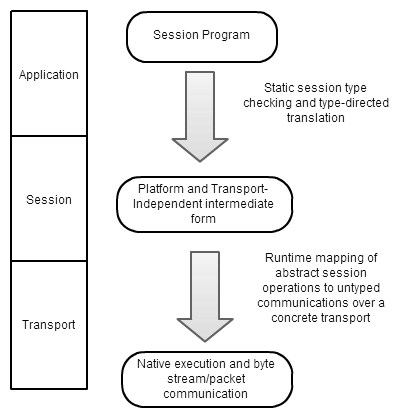
\includegraphics[width=0.7\textwidth]{resources/concept_sj_framework.png}
    \caption{Compilation and runtime stages of the Framework}
    \label{fig:image1}
\end{figure}

Figure \ref{fig:image1} depicts the compilation and runtime stages of the Framework, which operate across the layered architecture (session program, interaction services, abstract transport) just discussed. Below there is a brief description of each layer.

\begin{description}
\item[Application Layer] \hfill \\
The SJ Framework offers the application programmer a rich language facility for transport-independent object-oriented session programming. The compiler, statically type checks programs, and generates a transport-independent intermediate form by translating session operations into calls to the interaction services.

\item[Session Layer] \hfill \\
The Runtime has two main responsibilities. The first is performing the interaction services over the Abstract Transport. Services are incorporated into the Runtime as service components. Example: services include session initiation (which validates session peer compatibility), the wire format and serialization for communicating session messages, and cross-transport session migration for delegation as mentioned above.

\item[Abstract Transport Layer] \hfill \\
The second role of the Runtime is managing concrete connections, established using available transports, to realize the semantics of the Abstract Transport. The Abstract Transport operations are executed as actions on the underlying transports as directed by transport module implementations.
\end{description}

\section{Outline of the Thesis}

The remainder of this thesis is structured as follows:

\begin{description}
\item[Chapter \ref{chap:fundamentals}: Fundamentals] \hfill \\
Chapter \ref{chap:fundamentals} gives a background information that helps to understand the design decisions and formal model. The section include short introductions into the following topics: integration middlewares, service-oriented architectures, general standards for Web-service composition, and summarizes the papers that is fundamental to understand the session-based communication.

\item[Chapter \ref{chap:formal-theory}: Formal Theory] \hfill \\
Chapter \ref{chap:formal-theory} presents the formal theory of session-based communication structured concurrent programming, that was developed by Nobuko Yoshida, Kohei Honda, Robin Milner and Marco Carbone. The formal theory describes the global interaction as well as end-point behaviours by providing syntax, reduction rules and typing rules.

\item[Chapter \ref{chap:session-based-programming}: Session-based programming and business protocols] \hfill \\
Chapter \ref{chap:session-based-programming} is an implementation part of different business scenarios on e-commerce portal v3na.com. Each scenario consists of interactions and protocol definition, implementation and conclusion parts. The goal of this chapter is to confirm the suitability and applicability of formal theory based on session types.

\item[Chapter \ref{chap:evaluation}: Evaluation] \hfill \\
Chapter \ref{chap:evaluation} presents the evaluation of the Session-Java by comparing it with Java RMI. Highlights the realization of the most important concepts of session programming.

\item[Chapter \ref{chap:conclusion}: Conclusion] \hfill \\
Chapter \ref{chap:conclusion} concludes the thesis with a summary and an outlook on future work.
\end{description}